\documentclass[12pt,letterpaper]{article}

\usepackage{tikz}
\usetikzlibrary{shapes}

\usepackage{amssymb,amsmath,amsthm}
\usepackage{enumerate}
\usepackage[margin=1.25in]{geometry}
\usepackage{graphicx,ctable,booktabs}
\usepackage{fancyhdr}
\usepackage[utf8]{inputenc}
\usepackage{siunitx}

\makeatletter
\newenvironment{problem}{\@startsection
       {section}
       {1}
       {-.2em}
       {-3.5ex plus -1ex minus -.2ex}
       {2.3ex plus .2ex}
       {\pagebreak[3]
       \large\bf\noindent{Problem }
       }
       }
\makeatother

\renewcommand{\thesection}{\Roman{section}}

\title{Quiz $2$: Geometry}
\author{Name: \underline{\hspace{5cm}} Mark: $\displaystyle \frac{\hspace{3em}}{14}$}
\date{May 8, 2015}

\pagestyle{fancy}
\lhead{Quiz $2$: Geometry}
\chead{} 
\rhead{\thepage} 
\lfoot{\small\scshape Grade 4 Olympic Math} 
\cfoot{} 
\rfoot{}
\renewcommand{\headrulewidth}{.3pt} 
\renewcommand{\footrulewidth}{.3pt}
\setlength\voffset{-0.25in}
\setlength\textheight{648pt}
\setlength\headheight{15pt}

\newcommand*\circleletter[1]{%
  \begin{tikzpicture}[baseline=(C.base)]
    \node[draw,circle,inner sep=1pt](C) {#1};
  \end{tikzpicture}}

\begin{document}

\maketitle

\thispagestyle{empty}

There are no perfect right angles in nature.
For this quiz, assume that all angles that look right are right, and that all lines
that look parallel are parallel.

\begin{problem}{Toronto}
\begin{figure}[h]
  \begin{center}
    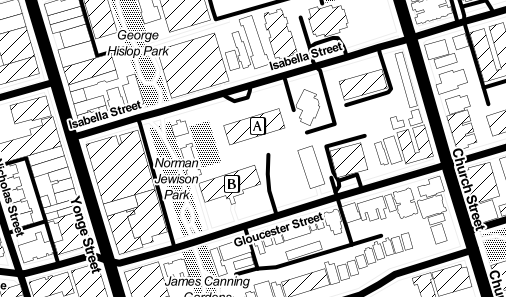
\includegraphics[width=.7\textwidth]{toronto.png}
  \end{center}
  \caption{Map from OpenStreetMap}
\end{figure}

 Look at the map of this block in Toronto. Answer the following questions by
 circling the best response, or if there is more than one correct response,
 \emph{\textbf{circle all correct responses}}.
 
 \begin{enumerate}
  \item At what kind of angle do Isabella Street and Church Street intersect?
  
  \hfill Acute~~Right~~Obtuse~~Straight~~Reflex
  
  \item What kind of shape is Building~\circleletter{A}?  
  \hfill Square~~Rectangle~~Parallelogram
  
  \item What is the sum of interior angles for Building~\circleletter{A}?
  \hfill $90^\circ$~~$180^\circ$~~$360^\circ$~~$540^\circ$
  
  \item Which building has greater area?  
  \hfill Building~\circleletter{A}~~Building~\circleletter{B}
 \end{enumerate}
\end{problem}

\begin{problem}{Swimming Pool}
 A rectangular swimming pool has length \SI{25}{\meter} and width \SI{20}{\meter}.
 
 \begin{enumerate}
  \item What is its area?
  \hfill \underline{\hspace{3em}} \si{\meter^2}
  
  \item Is the swimming pool a square? (circle one) \hfill Yes~~No
 \end{enumerate}
\end{problem}

\begin{problem}{Garden}
\begin{figure}[h]
  \begin{center}
    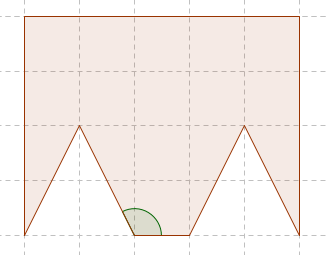
\includegraphics[width=.6\textwidth]{garden.png}
  \end{center}
\end{figure}

 Look at the map of Vegeta's vegetable garden. The shaded part is the
 garden itself. Each grid square represents \SI{1}{\meter^2}. One angle is marked.
 
 \begin{enumerate}
  \item What kind of angle is the marked angle? (circle one)
  
  \hfill Acute~~Right~~Obtuse~~Straight~~Reflex
  
  \item The angle supplementary to the marked angle is $63^\circ$.
  What is the measure of the marked angle?
  
  \hfill $\underline{\hspace{3em}}^\circ$

  \item How many sides does this garden have? \hfill $\underline{\hspace{3em}}$

  \item How many of the garden's interior angles are reflex angles?
  \hfill $\underline{\hspace{3em}}$
  
  \item What is the area of this garden? \hfill $\underline{\hspace{3em}}$ \si{\meter^2}
 \end{enumerate}

\end{problem}

\begin{problem}{Challenge}
 Two angles are complementary. One is $20^\circ$ greater than the other.
 What are the two angles?
 
 \hfill $\underline{\hspace{3em}}^\circ$, $\underline{\hspace{3em}}^\circ$
\end{problem}


\end{document}